\documentclass[12pt,a5paper,fleqn]{article}
\usepackage[utf8]{inputenc}
\usepackage{amssymb, amsmath, multicol}
\usepackage[russian]{babel}
\usepackage{graphicx}
\usepackage[shortcuts,cyremdash]{extdash}
\usepackage{wrapfig}
\usepackage{floatflt}
\usepackage{lipsum}
\usepackage{concmath}
\usepackage{euler}
\usepackage{tabto}
\usepackage{indentfirst}
%\usepackage{mathabx}
%\changenotsign

\graphicspath{ {images/} }

\oddsidemargin=-17.9mm
\textwidth=133mm
\headheight=-37mm
\textheight=210mm
\tolerance=100
\parskip=6pt
\pagestyle{empty}
\renewcommand{\tg}{\mathop{\mathrm{tg}}\nolimits}
\renewcommand{\ctg}{\mathop{\mathrm{ctg}}\nolimits}
\renewcommand{\arctan}{\mathop{\mathrm{arctg}}\nolimits}
\newcommand{\divisible}{\mathop{\raisebox{-2pt}{\vdots}}}
\renewcommand{\not}{\overline}

\renewcommand\neq{\mathrel{\vphantom{|}\mathpalette\xsneq\relax}}
\newcommand\xsneq[2]{%
  \ooalign{\hidewidth$#1|$\hidewidth\cr$#1=$\cr}%
}




\author{Старченко Иван}
\title{Лабораторная работа 1.2.4\\ Определение главных мометов инерции твердых тел с помощью крутильных колебаний }
\date{26 ноября 2020 г.}


\begin{document}

\maketitle
\newpage

\begin{center}
\begin{LARGE}
Теория:
\end{LARGE}
\end{center}

Введем некоторые основные определения:

 \textbf{Вращательное движение} -- вид механического движения. При вращательном движении материальная точка описывает окружность. При вращательном движении абсолютно твёрдого тела все его точки описывают окружности, расположенные в параллельных плоскостях. Центры всех окружностей лежат при этом на одной прямой, перпендикулярной к плоскостям окружностей и называемой \textbf{осью вращения}. Ось вращения может располагаться внутри тела и за его пределами. Ось вращения в данной системе отсчёта может быть как подвижной, так и неподвижной.
 
Инерционное свойство твердого тела при вращении определяет не только величина его массы но и её пространственное распределение. Последнее характеризует физическая величина которая называется тензором инерции.Рассмотрим момент импульса тела относительно центра масс.\\
\[\vec{L}=\displaystyle\sum_im_i\vec{r_i}\times\vec{v_i}\]

Поскольку при вращении тела относительно неподвижной точки скорости его точек даются выраженем $\vec{v_i} = \vec{\omega}\times \vec{r_i}$, то двойное вектрное произведение преобразовано по праавилу: \\
${\vec{a}} \cdot ({\vec{b}} \cdot {\vec{c}}) = \vec{b}\mbox{ } (\vec{a}\cdot \vec{c}) - \vec{c}\mbox{ } ({\vec{a}} \cdot {\vec{b}})$:\\
\[\vec{L}=\displaystyle\sum_i m_i\vec{r_i}\times(\vec{\omega}\times \vec{r_i}) = \sum_i m_i \big[ \vec{\omega}\mbox{ } \vec{|r_i|}^2 - \vec{r_i} (\vec{\omega}\cdot \vec{r_i})\big]\]

	Из этого равенства в общем случае видно, что векторы $\vec{L}$ и $\vec{\omega}$ не параллельны.
	
	Запишем полученное равенство в прямоугольных координатах:
	
\mbox{ }\mbox{ }\mbox{ }$L_x = \displaystyle \sum_i m_i\big[(x_i^2+y_i^2+z_i^2)\omega_x - (x_i\omega_x+y_i\omega_y+z_i\omega_z)x_i\big] =  \\ = \Big[ \sum_i m_i (y_i^2+z_i^2)\Big]\omega_x + \Big[ \sum_i(-m_ix_iy_i) \Big]\omega_y + \Big[\sum_y(-m_ix_iz_i)\Big]\omega_z $.

\newpage

	C помощью циклической замены~(~$x\rightarrow y\rightarrow z \rightarrow x$~)~ полчуимм другие компоненты вектора момента импульса. В итоге:\\
$L_x = \Big[ \sum_i m_i (y_i^2+z_i^2)\Big]\omega_x + \Big[ \sum_i(-m_ix_iy_i) \Big]\omega_y + \Big[\sum_y(-m_ix_iz_i)\Big]\omega_z $\\
$L_x = \Big[ \sum_i (-m_i y_i x_i)\Big]\omega_x + \Big[ \sum_im_i( z_i^2+x_i^2 ) \Big]\omega_y + \Big[\sum_y(-m_iy_iz_i)\Big]\omega_z $\\
$L_x = \Big[ \sum_i (-m_i z_ix_i)\Big]\omega_x + \Big[ \sum_i(-m_iz_iy_i) \Big]\omega_y + \Big[\sum_y m_i (x_i^2+z_i^2)\Big]\omega_z $

	Перепишем неравенства в следующей форме:\\
$L_x = I_{xx}\omega_x+I_{xy}\omega_y+I_{xz}\omega_z$\\
$L_y = I_{yx}\omega_x+I_{yy}\omega_y+I_{yz}\omega_z$\\
$L_z = I_{zx}\omega_x+I_{zy}\omega_y+I_{zz}\omega_z$

	Перепишем в матричном виде:	
\begin{equation*}
\begin{pmatrix}
L_x \\
L_y \\
L_z 
\end{pmatrix} 	
	=
	\begin{pmatrix}
	I_{xx} & I_{xy} & I_{xz} \\
	I_{yx} & I_{yy} & I_{yz} \\
	I_{zx} & I_{zy} & I_{zz}
	\end{pmatrix} 	
	\cdot	 
	\begin{pmatrix}
	\omega_x \\
	\omega_y \\
	\omega_z 
	\end{pmatrix}
\end{equation*}

Матрица:
\begin{equation*}
\stackrel{\land}{I}
	=
	\begin{pmatrix}
	I_{xx} & I_{xy} & I_{xz} \\
	I_{yx} & I_{yy} & I_{yz} \\
	I_{zx} & I_{zy} & I_{zz}
	\end{pmatrix} 	
		=
		\begin{pmatrix}
		\sum_i m_i (y_i^2+z_i^2) & -\sum_i m_i x_i y_i & 			-\sum_i m_i x_i z_i \\
		-\sum_i m_i y_i x_i & \sum_i m_i (z_i^2+y_i^2) & 
		-\sum_i m_i y_i z_i \\
		-\sum_i m_i y_i x_i & -\sum_i m_i z_i y_i & 
		\sum_i m_i (x_i^2+z_i^2) \\
		\end{pmatrix}
\end{equation*}
называется тензором инерции.

Пусть вектор угловой скорости направлен вдоль оси $x$: $\vec{\omega} = \vec{i} \omega_x$. Тогда $L_x = I_{xx}\omega_x$. Это означает, что величина $I_{xx}$ представляет собой момент инерции тела
при вращении относительно оси $х$, т.~е. $I_{xx} = I_x$ . Аналогично, величины
$I_{yy}= I_y,  I_{zz} = I_z$ представляют собой соответствующие осевые моменты
инерции.

Недиагональные компоненты тензора инерции называют центробежными моментами инерции.
Из определения видно, что тензор инерции является симметричным,
то есть $I_{ik} = I_{kj}$. Более подробно это записывается в виде
$I_{xy} = I_{ух},  I_{xz} = I_{zx}, I_{yz} = I_{zy}$.
Таким образом, имеется всего $6$ существенных компонент тензора инерции: три диагональные и три недиагональные.

\newpage

Если для какой-лтбо системы координат известны все шесть элементов матрицы, то момент инерции тела относительно произвольной оси, проходящей через начало координат, может быть вычислен по формуле:
\[I = I_{xx}e_x^2+I_{yy}e_y^2+I_{zz}e_z^2+2I_{xy}e_xe_y+2I_{yz}e_ye_z+2I_{xz}e_xe_z,\] где $e_x, e_y,e_z -- $координаты единичного вектора $\vec{e}$ и
\begin{equation*}
\begin{matrix}
	I_{xx} = -\int (e_y^2 +e_z^2) dm & I_{xy} = 			I_{yx} = \int e_xe_ydm\\
	I_{yy} = -\int (e_z^2 +e_x^2) dm & I_{yz} = 			I_{zy} = \int e_ze_ydm\\
	I_{zz} = -\int (e_x^2 +e_y^2) dm & I_{xz} = 			I_{zx} = \int e_xe_zdm
	\end{matrix} 
\end{equation*}
	\hspace{0.5cm}Как и всякая симметричная матрица, матрица тензора инерции может быть приведена к диагональному
виду, диагональные элементы $I_x, I_y, I_z$ которой называются главными моментами инерции тела. Геометрическим образом тензора инерции является эллипсонд, уравнение которого в главных осях имеет вид:
\[I_x x^2 + I_y y^2+ I_z z^2 = 1\]

	Этот эллиисоид принято называть эллипсоидом инерции. Эллипсоид инерции жестко связан с телом, для которого построен. Координатные оси $Ox, Oy, Oz$ совпадают с главными осями тела. Если начало
координат $O$ совпадает с центром масс тела, то эллипсонд инерции называется центральным.

	Знание эллинсоида инерции позволяет найти момент инерции тела относительно любой оси, проходившей через центр эллиисоида. Для этого необходимо вдоль выбранной оси провести радиус-вектор  до пересечения с поверхностью эллипсоида. Длина $\vec{r}$ будет определять момент инерции тела относительно этой оси:
\[I = \dfrac{1}{r^2}\]

	Главные оси тела часто можно определить из
его симметрии. Например, оси симметрии цилиндра или шара являются главными осями, так как для всех осей, лежащих в плоскости перпендикулярной оси симметрии, моменты инерции одинаковые, и, следовательно,

\newpage 

\noindent эллипсоид инерции обладает такой же симметрией, являясь эллипсоидом вращения относительно оси симметрии тела.

	Эллипсоид инерции оказывается симметричным и для некоторых тел, не обладающих осевой симметрией. Например, для прямоугольного параллелепипеда с квадратным основанием и для кубика. Для последнего эллипсоид превращаетсz в сферическую поверхность, из чего следует, что величина момента инерции не зависит от направления оси, так же как в случае шара. 
	
	На рисунке $1$ для прямоугольного параллелепипеда, диска и кубика нарисованы (в произвольном масштабе) центральные эллипсоиды инерции.
	
\begin{center}
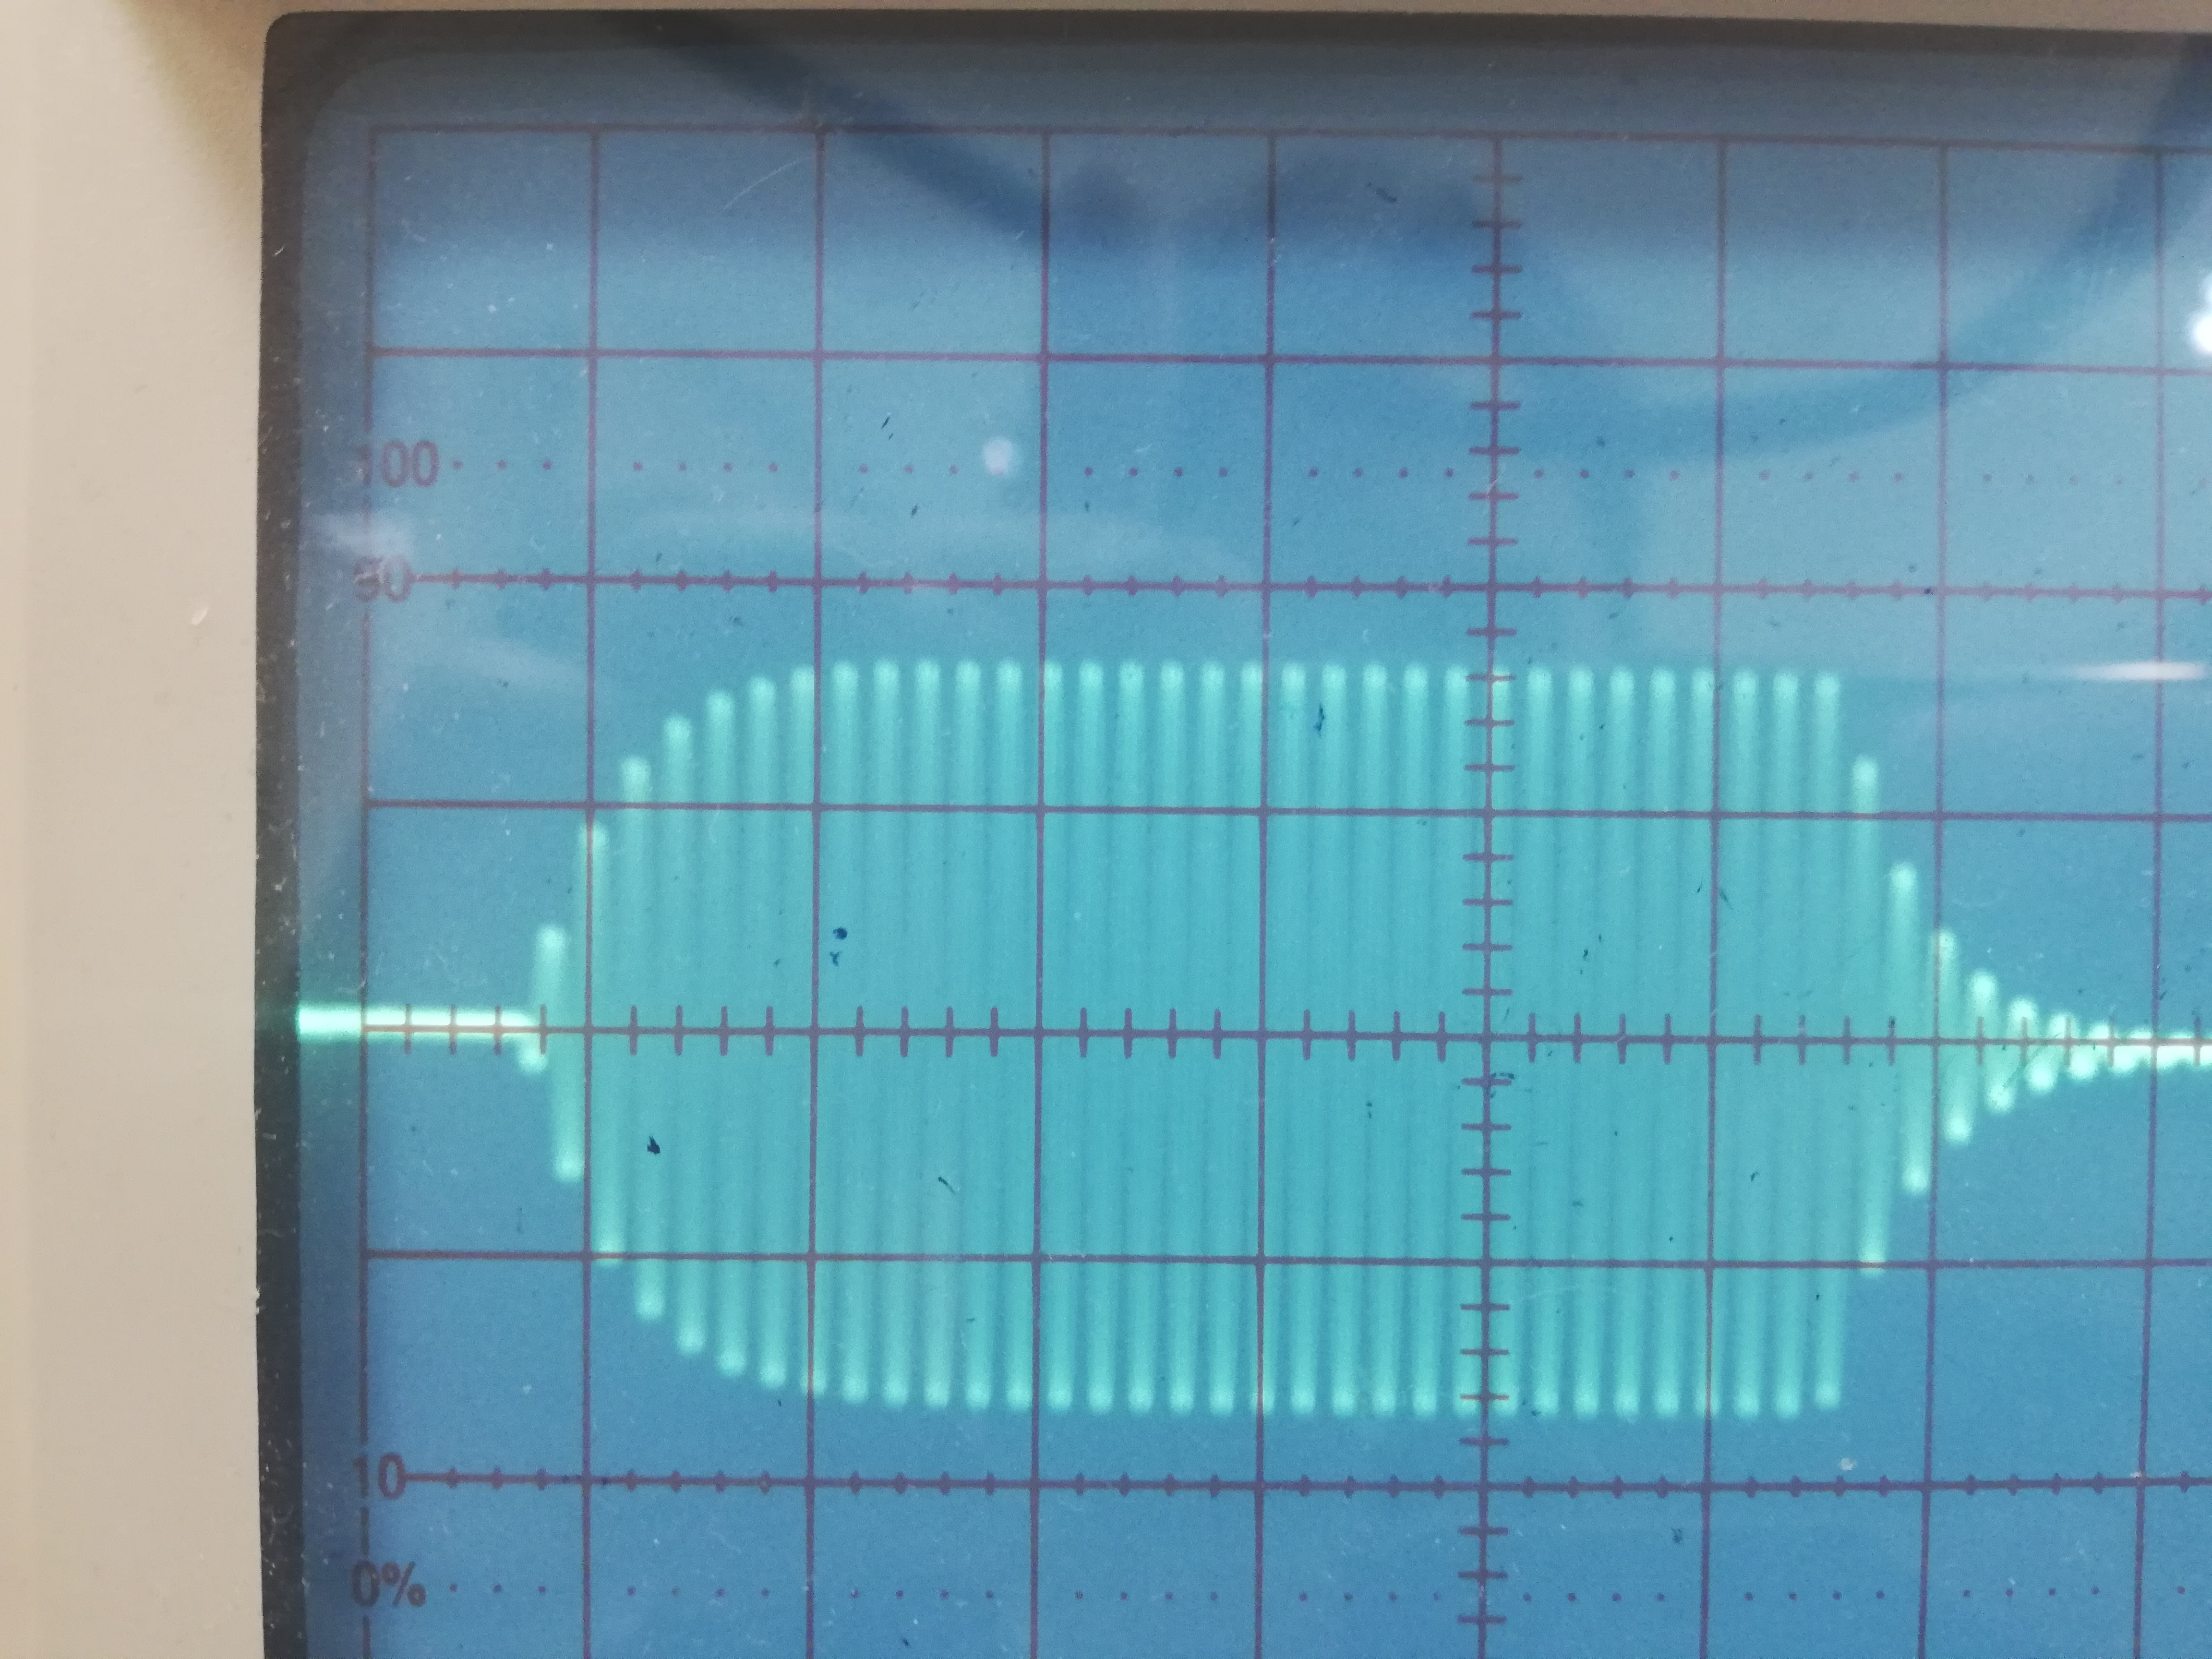
\includegraphics{2}
\end{center}
	\hspace{0.5cm}По теореме Кёнига кинетическая энергия системы материальных точек в лабораторной системе отсчёта даётся выражением
\[K_{system} = \dfrac{mv_c^2}{2}+ K\]

\newpage

где $m$ -- суммарная масса системы, $v_c$ -- скорость центра масс системы, а $K$ -- кинетическая энергия точек системы. относительно центра масс. Последнее слагаемое в случае твёрдого тела сводится к вращению тела как целого. Если $v_i$, -- скорость $i$-й точки относительно центра масс, то
\[K = \dfrac{m_i v_i^2}{2}\]
	Cкорость $v_i$, можно представить в виде
\[\vec{v_i} = \vec{\omega} \times \vec{r_i}\]
	\hspace{0.5cm}Подстановки этого выражения в формулу кинетической энергии точек даёт
\[K = \dfrac{m_i}{2}(\omega \times r_i)^2\]
	Также учтем тождество 
\[(\vec{\omega} \times \vec{r_i})^2 = \omega^2 r_i^2 sin^2 \varphi = \omega^2 r_i^2 (1-cos^2\varphi) = \omega^2 r_i^2 - (\vec{\omega}\cdot\vec{r_i})^2\]
	Поэтому получаем 
\[K = \sum_i \dfrac{m_i}{2}\Big[\omega^2 r_i^2 - (\vec{\omega}\cdot\vec{r_i})^2\Big] =  \dfrac{1}{2}\vec{\omega} \sum_i m_i\Big[\vec{\omega}r_i^2 -(\vec{\omega} \vec{r_i})\vec{r_i} \Big] = \dfrac{1}{2}\vec{\omega}\vec{L},\]
где мы использовалт выражение для момента импульса тела 
\[L=\sum_i m_i\Big[\vec{\omega} r_i^2 - (\vec{\omega}\vec{r_i})\vec{r_i} \Big] = \sum_i m_i\vec{ r} \times (\vec{\omega}\times \vec{r_i}) = \sum_i m_i \vec{r} \times \vec{v_i} \]
	\hspace{0.5cm}Имея в виду связь момента импульса с угловой скоростью, перепишем выражение для кинетической энергии тела в виде
\[K=\dfrac{1}{2}\Big(\vec{\omega},\stackrel{\land}{I}\vec{\omega}\Big)\]
Если $x,y$ и $z$ -- главные оси инерции, то 
\[K =\dfrac{1}{2}\Big(I_x\omega_x^2+I_y\omega_y^2+I_z\omega_z^2\Big)\]

\newpage

В общем случае при вращении тела его главные оси также совершают поворот в пространстве. Это следует учитывать при записи уравнений, определяющих закон изменения компонент вектора угловой скорости со временем.





\end{document}